\documentclass{beamer}

\usepackage{etex}
\usepackage{stmaryrd}
\usepackage{color}
\usepackage{geometry}
\usepackage[utf8]{inputenc}
\usepackage{amsmath}
\usepackage{bussproofs}
\usepackage{graphicx}
\usepackage{tabularx}
\usepackage{changepage}
\usepackage{listings}
\usepackage{amssymb}
\usepackage{amsthm}
\usepackage{mathtools}
\usepackage{tikz}


\usetikzlibrary{matrix, positioning, arrows, decorations, decorations.pathreplacing, trees}

	\tikzset{
		table nodes/.style={
			rectangle,
			draw=black,
			align=center,
			minimum height=7mm,
			text depth=0.5ex,
			text height=2ex,
			inner xsep=0pt,
			outer sep=0pt
		},
		invisible/.style={opacity=0},
		visible on/.style={alt=#1{}{invisible}},
		alt/.code args={<#1>#2#3}{%
			\alt<#1>{\pgfkeysalso{#2}}{\pgfkeysalso{#3}} % \pgfkeysalso doesn't change the path
		},
		table/.style={
			matrix of nodes,
			row sep=\pgflinewidth,
			column sep=\pgflinewidth,
			nodes={
				table nodes
			},
			execute at empty cell={\node[draw=none]{};}
		}
	}


\usetheme{Copenhagen}


\beamertemplatenavigationsymbolsempty

\AtBeginSection[]
{
  \begin{frame}
    \frametitle{Agenda}
    \tableofcontents[currentsection]
  \end{frame}
}
\newcommand*\oldmacro{}%
\let\oldmacro\insertshorttitle%
\renewcommand*\insertshorttitle{%
  \oldmacro\hfill%
  \insertframenumber\,/\,\inserttotalframenumber}

\setbeamertemplate{bibliography item}{}

\begin{document}
\author[Christoph Welzel]{Christoph Welzel}
\date{Januar 08, 2015}
\title{Permission Accounting in Separation Logic}
\begin{frame}
	\maketitle
\end{frame}

\begin{frame}
	\tableofcontents
\end{frame}

\section{Introduction}
	\begin{frame}
	\frametitle{Introduction}
	\begin{itemize}
		\item importance of automated verification of programs increases
		\item performance improvement due to concurrent execution
		\item concurrency $\rightarrow$ \emph{race-conditions}, \emph{shared-memory}, \dots
		\begin{itemize}
			\item manage access $\rightarrow$ reading vs. writing
		\end{itemize}
		\item approached by extending well-known techniques (i.e. \emph{Hoare Calculus})
	\end{itemize}
	\end{frame}
\section{Hoare Calculus}
		\begin{frame}
			\frametitle{General}
			\begin{itemize}
				\item logical reasoning about programs given by source code
				\item logical assertions for states
					\begin{itemize}
						\item \emph{Precondition} and \emph{Postcondition}
					\end{itemize}
				\item (automated) verification of programs
			\end{itemize}
		\end{frame}

		\begin{frame}
			\frametitle{Use of \emph{Hoare Calculus}}
			\begin{block}{\emph{Hoare Triple}: Unit of \emph{Hoare Calculus}}
				$$\{P\}Q\{R\}$$
				\begin{itemize}
					\item Precondition: $P$
					\item Program: $Q$
					\item Postcondition: $R$
				\end{itemize}
			\end{block}
		\end{frame}

		\begin{frame}
			%tf?
			\frametitle{Properties of \emph{Hoare triple}}
			\begin{block}{\emph{Partial Correctness}}
				$$\{P\}Q\{R\}$$
				given $P$, $R$ holds after the execution of $Q$.
			\end{block}
			\begin{itemize}
				\item apply rules and axioms to prove \emph{Partial Correctness}
				\item beware of non-terminating programs
			\end{itemize}
			\begin{block}{\emph{Total Correctness}}
				$$\{P\}Q\{R\}$$
				is \emph{partially correct} and $Q$ \emph{terminates}.
			\end{block}
		\end{frame}

		\begin{frame}
			\frametitle{\emph{Axiom of Assignment}}
			\begin{itemize}
				\item $x := E$
				\item valid assertion after assignment was true before
				\item scheme for proving assignment statements
				\item replace all occurences of $x$ by $E$
			\end{itemize}
			\begin{block}{\emph{Axiom of Assignment}}
				$$\{P[E/x]\}x := E\{P\}$$
				is \emph{partially correct}.
			\end{block}
		\end{frame}

		\begin{frame}[fragile]
			\frametitle{Example of \emph{Axiom of Assignment}}
			\begin{block}{\emph{Axiom of Assignment}}
				$$\{P[E/x]\}x := E\{P\}$$
				is \emph{partially correct}.
			\end{block}
			\begin{exampleblock}{Example}
				\begin{lstlisting}[mathescape]
					$\{x+1 > 0\}$
					 x := x + 1;
					$\{x > 0\}$
				\end{lstlisting}
			\end{exampleblock}
		\end{frame}

		\begin{frame}
		\frametitle{\emph{Rule of Composition}}
			\begin{itemize}
				\item programs consist of multiple commands
				\item executed sequentially
				\item program $Q_1$ gives \emph{postcondition} $T$
				\item program $Q_2$ needs \emph{precondition} $T$
				\item $Q_1; Q_2$ can be reasoned about individually
			\end{itemize}
			\begin{block}{\emph{Rule of Composition}}
				\begin{prooftree}
					\AxiomC{$\{P\}Q_1\{T\}$}
					\AxiomC{$\{T\}Q_2\{R\}$}
					\BinaryInfC{$\{P\}Q_1; Q_2\{R\}$}
				\end{prooftree}
			\end{block}
		\end{frame}

		\begin{frame}[fragile]
		\frametitle{Example of \emph{Rule of Composition} I}
			\begin{block}{\emph{Rule of Composition}}
				\begin{prooftree}
					\AxiomC{$\{P\}Q_1\{T\}$}
					\AxiomC{$\{T\}Q_2\{R\}$}
					\BinaryInfC{$\{P\}Q_1; Q_2\{R\}$}
				\end{prooftree}
			\end{block}

			\begin{exampleblock}{Example}
			\begin{minipage}[t]{0.51\textwidth}
				\begin{lstlisting}[mathescape]
					$\{1337 = 1337$
					 $\land (1337-1295) = 42\}$
					 x := 1337;
					$\{x = 1337 \land (x-1295) = 42\}$
				\end{lstlisting}
			\end{minipage}\noindent
			\hfill
			\vline
			\hfill
			\begin{minipage}[t]{0.48\textwidth}
				\begin{lstlisting}[mathescape]
					$\{x = 1337 \land (x-1295) = 42\}$
					 y := x-1295;
					$\{x = 1337 \land y = 42\}$
				\end{lstlisting}
			\end{minipage}
			\end{exampleblock}
		\end{frame}

		\begin{frame}[fragile]
		\frametitle{Example of \emph{Rule of Composition} II}
		\begin{exampleblock}{Example}
			\begin{minipage}[t]{0.51\textwidth}
				\begin{lstlisting}[mathescape]
					$\{1337 = 1337$
					 $\land (1337-1295) = 42\}$
					 x := 1337;
					$\{x = 1337 \land (x-1295) = 42\}$
				\end{lstlisting}
			\end{minipage}\noindent
			\hfill
			\vline
			\hfill
			\begin{minipage}[t]{0.48\textwidth}
				\begin{lstlisting}[mathescape]
					$\{x = 1337 \land (x-1295) = 42\}$
					 y := x-1295;
					$\{x = 1337 \land y = 42\}$
				\end{lstlisting}
			\end{minipage}
			\rule{\textwidth}{1pt}
			\begin{minipage}{0.28\textwidth}
				\hfill
			\end{minipage}\noindent
			\begin{minipage}{0.3\textwidth}
			\begin{lstlisting}[mathescape]
				$\{1337 = 1337$
				 $\land (1337-1295) = 42\}$
				 x:=1337;
				 y:=x-1295;
				$\{x = 1337 \land y = 42\}$
			\end{lstlisting}
			\end{minipage}
		\end{exampleblock}
		\end{frame}

		\begin{frame}
		\frametitle{\emph{Rule of Consequence}}

		\begin{itemize}
			\item logical implication for assertions
			\item strengthen \emph{preconditions}
			\item weaken \emph{postconditions}
		\end{itemize}
		\begin{block}{\emph{Rule of Consequence}}
			\begin{prooftree}
				\AxiomC{$\{S\}\therefore \{P\}$}
				\AxiomC{$\{P\}Q\{S'\}$}
				\AxiomC{$\{S'\}\therefore \{R\}$}
				\TrinaryInfC{$\{S\}Q\{R\}$}
			\end{prooftree}
			\begin{itemize}
				\item logical implication of assertions: $\therefore$
			\end{itemize}
		\end{block}

		\end{frame}


		\begin{frame}[fragile]
		\frametitle{Example of \emph{Rule of Consequence}}

		\begin{block}{\emph{Rule of Consequence}}
			\begin{prooftree}
				\AxiomC{$\{S\}\therefore \{P\}$}
				\AxiomC{$\{P\}Q\{S'\}$}
				\AxiomC{$\{S'\}\therefore \{R\}$}
				\TrinaryInfC{$\{S\}Q\{R\}$}
			\end{prooftree}
		\end{block}
		\begin{exampleblock}{Example}
			\begin{minipage}{0.5\textwidth}
				\begin{lstlisting}[mathescape]
					$\{1 = 1\}$ x := 1; $\{x = 1\}$
				\end{lstlisting}
			\end{minipage}\noindent\vline
			\begin{minipage}{0.5\textwidth}
				$$\{x = 1\} \therefore \{x > 0\}$$
			\end{minipage}
			\rule{\textwidth}{1pt}
			\begin{minipage}{0.42\textwidth}
			\hfill
			\end{minipage}\noindent
			\begin{minipage}{0.58\textwidth}
			\begin{lstlisting}[mathescape]
				$\{1 = 1\}$
				 x := 1;
				$\{x > 0\}$
			\end{lstlisting}
			\end{minipage}
		\end{exampleblock}

		\end{frame}


		\begin{frame}[fragile]
		\frametitle{Example of \emph{Rule of Consequence}}

		\begin{block}{\emph{Rule of Consequence}}
			\begin{prooftree}
				\AxiomC{$\{S\}\therefore \{P\}$}
				\AxiomC{$\{P\}Q\{S'\}$}
				\AxiomC{$\{S\}'\therefore \{R\}$}
				\TrinaryInfC{$\{S\}Q\{R\}$}
			\end{prooftree}
		\end{block}
		\begin{exampleblock}{Alternativ writing}
		\begin{minipage}{0.42\textwidth}
		\hfill
		\end{minipage}\noindent
		\begin{minipage}{0.58\textwidth}
		\begin{center}
		\begin{lstlisting}[mathescape]
			$\{1 = 1\}$
			 x := 1;
			$\{x = 1\}$
		$\therefore\{x > 0\}$
		\end{lstlisting}
		\end{center}
		\end{minipage}
		\end{exampleblock}

		\end{frame}


		\begin{frame}
		\frametitle{\emph{Rule of Iteration}}

		\begin{itemize}
			\item loops, iterations
			\item proof of properties via \emph{invariant}
			\item \emph{invariant} holds for every execution of loop-body
		\end{itemize}

		\begin{block}{\emph{Rule of Iteration}}
			\begin{prooftree}
			\AxiomC{$\{I\land B\}C\{I\}$}
			\UnaryInfC{$\{I\}\textit{while $B$ do $C$ od}\{\lnot B\land I\}$}
			\end{prooftree}
		\end{block}

		\end{frame}

\section{Separation Logic}
	\subsection{Heap and Store}

	\begin{frame}
	\frametitle{Idea}

	\begin{itemize}
		\item separated representation of variables and dynamic memory
		\item defined by \emph{Store} and \emph{Heap}
		\item represents state of machine
	\end{itemize}

	\end{frame}


	\begin{frame}[fragile]
	\frametitle{\emph{Store}}

	\begin{itemize}
		\item maps variables to values
	\end{itemize}
	\begin{block}{\emph{Store}}
		$$s: \textit{Vars} \rightharpoonup \textit{Integers}$$
	\end{block}
	\begin{exampleblock}{Representation of a \emph{Store}}
	\begin{center}
	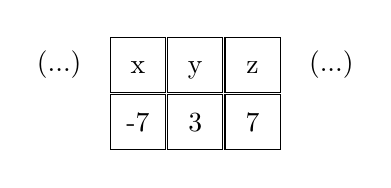
\begin{tikzpicture}
		\matrix (store) [table, text width=7mm, name=table]
			{ x & y & z \\
			 -7 & 3 & 7 \\ };
		\node (l) [left of=table-1-1] {(...)};
		\node (r) [right of=table-1-3] {(...)};
	\end{tikzpicture}
	\end{center}
	\end{exampleblock}

	\end{frame}


	\begin{frame}[fragile]
	\frametitle{\emph{Heap}}

	\begin{itemize}
		\item \emph{Heap}: dynamically managed memory
		\item possible representation: addressable cells
	\end{itemize}
	\begin{block}{\emph{Heap}}
		$$h: \mathbb{N} \rightharpoonup \textit{Integers}$$
	\end{block}
	\begin{exampleblock}{Representation of a \emph{Heap}}
	\begin{center}
	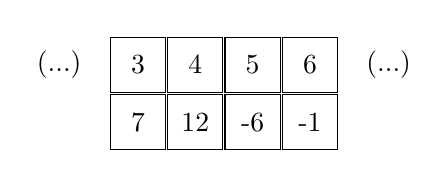
\begin{tikzpicture}
		\matrix (heap) [table, text width=7mm, name=table]
			{ 3 &  4 &  5 &  6 \\
			  7 & 12 & -6 & -1 \\ };
		\node (l) [left of=table-1-1] {(...)};
		\node (r) [right of=table-1-4] {(...)};
	\end{tikzpicture}
	\end{center}
	\end{exampleblock}

	\end{frame}


	\begin{frame}
	\frametitle{Properties of \emph{Store}}
		\begin{itemize}
			\item to this point: no difference between logical and programming variables
			\item from this point: programming variables interpreted by \emph{Store}
		\end{itemize}
		\begin{block}{Interpretation of expression}
			$$\llbracket E\rrbracket s = v$$
			\begin{itemize}
				\item \emph{Store}: $s$
				\item \emph{Expression}: $E$
				\item \emph{value}: $v$
			\end{itemize}
		\end{block}
	\end{frame}

	\begin{frame}
	\frametitle{Example for interpretations by \emph{Store}}
	\begin{block}{Interpretation of expression}
			$$\llbracket E\rrbracket s = v$$
	\end{block}

	\begin{exampleblock}{Interpretation of expressions}
		$x\in \textit{dom}(s)$
		\begin{itemize}
			\item $\llbracket x\rrbracket s = s(x)$
			\item $\llbracket (x + 1)\rrbracket s = s(x) + 1$
		\end{itemize}
	\end{exampleblock}

	\end{frame}

	\subsection{Operators}


	\begin{frame}[fragile]
	\frametitle{Content of cell}
		\begin{itemize}
			\item content of cell
			\item connect address with value
		\end{itemize}
		\begin{block}{$\mapsto$ operator}
			$$E \mapsto E'$$
			\vspace{-0.7cm}
			\begin{itemize}
				\item \emph{address}: $E, \llbracket E\rrbracket s\in\textit{dom}(h)$
				\item \emph{value}: $\llbracket E'\rrbracket s\in\textit{Integers}$
			\end{itemize}
			\begin{center}
			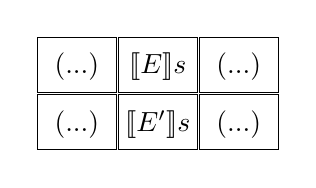
\begin{tikzpicture}
				\matrix (heap) [table, text width=10mm, name=table]
					{ (...) & $\llbracket E \rrbracket s$ & (...) \\
					  (...) & $\llbracket E'\rrbracket s$ & (...) \\ };
			\end{tikzpicture}
			\end{center}
		\end{block}
	\end{frame}

	\begin{frame}[fragile]
	\frametitle{Example of $\mapsto$}
	\begin{exampleblock}{$\mapsto$ example}
	\begin{minipage}{0.5\textwidth}
	\begin{center}
	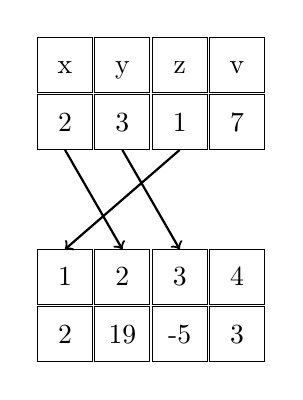
\begin{tikzpicture}
		\matrix (store) [table, text width=7mm, name=s]
			{ x & y & z & v \\
			  2 & 3 & 1 & 7 \\ };
		\matrix (heap) [table, text width=7mm, name=h, below=of s]
			{ 1 & 2 & 3 & 4 \\
			  2 &19 &-5 & 3 \\ };
		%arrows:
		\draw[thick,->] (s-2-1.south) -- (h-1-2.north);
		\draw[thick,->] (s-2-2.south) -- (h-1-3.north);
		\draw[thick,->] (s-2-3.south) -- (h-1-1.north);

	\end{tikzpicture}
	\end{center}
	\end{minipage}\noindent
	\begin{minipage}{0.5\textwidth}
		\begin{itemize}
			\item $x\mapsto 19$
			\item $y\mapsto -5$
			\item $z\mapsto 2$
			\item $4\mapsto 3$
			\item $\llbracket v\rrbracket s = 7$
		\end{itemize}
	\end{minipage}
	\end{exampleblock}
	\end{frame}

	\begin{frame}
	\frametitle{Formal definition}
	\begin{block}{States satisfy assertion}
		$$(s,h)\models P$$
		\vspace{-0.7cm}
		\begin{itemize}
			\item \emph{Store}: $s$
			\item \emph{Heap}: $h$
			\item \emph{Assertion}: $P$
		\end{itemize}
	\end{block}
	\begin{block}{$\mapsto$}
		$$(s,h)\models E\mapsto F\text{ iff }\llbracket E\rrbracket s=\textit{dom}(h)\land h(\llbracket E\rrbracket s) = \llbracket F\rrbracket s$$
	\end{block}
	\end{frame}

	\begin{frame}[fragile]
	\frametitle{}
	\begin{block}{$\mapsto$}
		$$(s,h)\models E\mapsto F\text{ iff }\llbracket E\rrbracket s=\textit{dom}(h)\land h(\llbracket E\rrbracket s) = \llbracket F\rrbracket s$$
	\end{block}
	\begin{exampleblock}{Example}
	\begin{minipage}{0.5\textwidth}
		\begin{tikzpicture}
			\matrix (heap) [table, text width=7mm, name=h, below=of s]
				{ 1 \\
				 14 \\};
			\node (formula) [right of=h, xshift=0.3cm] {$\widehat{=}\; 1 \mapsto 14$};
		\end{tikzpicture}
	\end{minipage}\noindent
	\begin{minipage}{0.5\textwidth}
		\begin{tikzpicture}
			\matrix (heap) [table, text width=7mm, name=h, below=of s]
				{ 1 &  2 \\
				 14 & -3 \\};
			\node (formula) [right of=h, xshift=0.5cm] {$\widehat{=}\;$ ???};
		\end{tikzpicture}
	\end{minipage}
	\end{exampleblock}
	\end{frame}

	\begin{frame}
	\frametitle{Motivation $\ast$ operator}
	\begin{block}{$\mapsto$}
		$$(s,h)\models E\mapsto F\text{ iff }\alert{\llbracket E\rrbracket s=\textit{dom}(h)}\land h(\llbracket E\rrbracket s) = \llbracket F\rrbracket s$$
	\end{block}
	\begin{itemize}
		\item glue larger \emph{Heaps} together
	\end{itemize}
	\begin{block}{$\ast$ operator}
		\begin{center}
		\begin{tabular}{lcl}
		$(s,h)\models P\ast Q$ & iff & $\exists h_1,h_2.h_1\#h_2\land h_1\bullet h_2=h,$\\
		                       &     & $(s,h_1)\models P\land (s,h_2)\models Q$
		\end{tabular}
		\end{center}
		\begin{itemize}
			\item \emph{disjunctive domains}: $h_1\# h_2$
			\item \emph{disjunctive union}: $h_1\bullet h_2$
		\end{itemize}
	\end{block}
	\end{frame}

	\begin{frame}[fragile]
	\frametitle{Example for $\ast$}
	\begin{exampleblock}{Example for $\ast$}
	\begin{minipage}{0.4\textwidth}
	\begin{center}
	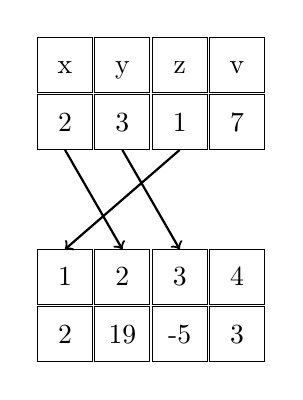
\begin{tikzpicture}
		\matrix (store) [table, text width=7mm, name=s]
			{ x & y & z & v \\
			  2 & 3 & 1 & 7 \\ };
		\matrix (heap) [table, text width=7mm, name=h, below=of s]
			{ 1 & 2 & 3 & 4 \\
			  2 &19 &-5 & 3 \\ };
		%arrows:
		\draw[thick,->] (s-2-1.south) -- (h-1-2.north);
		\draw[thick,->] (s-2-2.south) -- (h-1-3.north);
		\draw[thick,->] (s-2-3.south) -- (h-1-1.north);

	\end{tikzpicture}
	\end{center}
	\end{minipage}\noindent
	\begin{minipage}{0.6\textwidth}
		\begin{itemize}
			\item ${1 \mapsto 2} \ast {2 \mapsto 19} \ast {3 \mapsto -5} \ast {4 \mapsto 3}$
			\item ${(x-1) \mapsto 2} \ast {x \mapsto 19} \ast {y \mapsto -5} \ast {4 \mapsto 3}$
			\item \dots
		\end{itemize}
	\end{minipage}
	\end{exampleblock}

	\end{frame}


	\begin{frame}
	\frametitle{\textit{emp}}
	\begin{itemize}
		\item states of \emph{Heaps} can be expressed
		\item empty \emph{Heap}: \textit{emp}
		\item neutral element of $\ast$
		\item empty domain for $h$
	\end{itemize}
	\end{frame}

	\begin{frame}[fragile]
	\frametitle{\textit{swap} program}
	\begin{minipage}{0.4\textwidth}
	\begin{lstlisting}[mathescape]
	 swap($\text{ref}_1$, $\text{ref}_2$) {
	   tmp := new();
	   [tmp] := [$\text{ref}_1$];
	   [$\text{ref}_1$] := [$\text{ref}_2$];
	   [$\text{ref}_2$] := [tmp];
	   dispose(tmp);
	 }
	\end{lstlisting}
	\end{minipage}\noindent
	\begin{minipage}{0.6\textwidth}
		\begin{block}<2->{\emph{Axioms of Referenced Assignment}}
			\begin{minipage}{0.5\textwidth}
			\begin{lstlisting}[mathescape]
			$\{ E \mapsto - \}$
			 $[E] := F$
			$\{ E \mapsto F \}$
			\end{lstlisting}
			\end{minipage}\noindent
			\vline
			\begin{minipage}{0.5\textwidth}
			\begin{lstlisting}[mathescape]
			$\{E \mapsto n \land \llbracket x\rrbracket s = m\}$
			 $x := [E]$
			$\{\llbracket x \rrbracket s=n$
			   $\land E[m/x]\mapsto n\}$
			\end{lstlisting}
			\end{minipage}
			\rule{\textwidth}{1pt}
			\begin{minipage}{0.5\textwidth}
			\begin{lstlisting}[mathescape]
			$\{E \mapsto - \}$
			 $\textit{dispose}(E)$
			$\{\textit{emp}\}$
			\end{lstlisting}
			\end{minipage}\noindent
			\vline
			\begin{minipage}{0.5\textwidth}
			\begin{lstlisting}[mathescape]
			$\{\textit{emp}\}$
			 $x := \textit{new}()$
			$\{x\mapsto -\}$
			\end{lstlisting}
			\end{minipage}
		\end{block}
	\end{minipage}
	\end{frame}

	\begin{frame}[fragile]
	\frametitle{Locality of programs}
		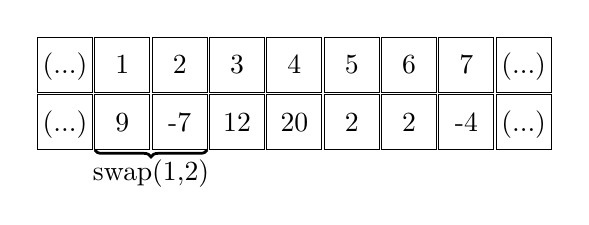
\begin{tikzpicture}[decoration={brace}]
			\matrix (heap) [table, text width=7mm, name=h]
				{ (...) &  1 &  2 &  3 &  4 &  5 &  6 &  7 & (...) \\
				  (...) &  9 & -7 & 12 & 20 &  2 &  2 & -4 & (...) \\};
			\draw [decorate, line width=1pt] (h-2-3.south east) -- (h-2-2.south west)
				node [midway, yshift=-0.3cm] {swap(1,2)};
		\end{tikzpicture}
		\begin{block}{\emph{Frame Rule}}
			\begin{prooftree}
				\AxiomC{$\{P\}C\{Q\}$}
				\RightLabel{$\textit{modifies}(C)\cap\textit{free}(R) = \emptyset$}
				\UnaryInfC{$\{P\ast R\}C\{Q\ast R\}$}
			\end{prooftree}
		\end{block}
	\end{frame}

	\subsection{Concurrency}

	\begin{frame}
	\frametitle{Concurrency}
	\begin{itemize}
		\item concurrently executed programs are possibly \emph{racy}
		\item Aim: guaranteed \emph{race-freedom} $\rightarrow$ proof for one schedule, not all possible
		\item 3 groups of \emph{race-free} access on variables:
			\begin{enumerate}[a)]
				\item variables read and written exclusively by one program
				\begin{itemize}
					\item[$\rightarrow$] \emph{Concurrency Rule}
				\end{itemize}
				\item shared memory accessed mutually-exclusive
				\begin{itemize}
					\item[$\rightarrow$] \emph{Conditional Critical Region}
				\end{itemize}
				\item shared memory which is only read 
				\begin{itemize}
					\item[$\rightarrow$] \emph{Permission Accounting}
				\end{itemize}
			\end{enumerate}
	\end{itemize}

	\end{frame}

	\begin{frame}[fragile]
	\frametitle{Syntax}
		\begin{block}{Concurrent Execution}
			$$C_1 \parallel C_2$$
			\vspace{-0.7cm}
			\begin{itemize}
				\item \emph{program}: $C_1, C_2$
			\end{itemize}
		\end{block}
		\begin{exampleblock}{Example}
			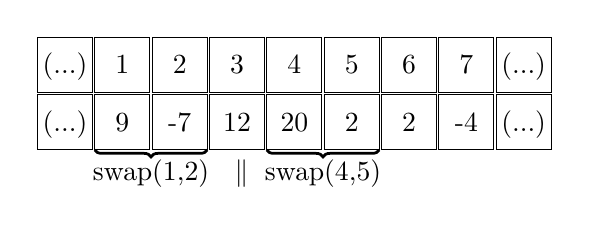
\begin{tikzpicture}[decoration={brace}]
			\matrix (heap) [table, text width=7mm, name=h]
				{ (...) &  1 &  2 &  3 &  4 &  5 &  6 &  7 & (...) \\
				  (...) &  9 & -7 & 12 & 20 &  2 &  2 & -4 & (...) \\};
			\draw [decorate, line width=1pt] (h-2-3.south east) -- (h-2-2.south west)
				node [midway, yshift=-0.3cm, name=t1] {swap(1,2)};
			\node (t2) [right of=t1, xshift=0.15cm] {$\parallel$};
			\draw [decorate, line width=1pt] (h-2-6.south east) -- (h-2-5.south west)
				node [midway, yshift=-0.3cm] {swap(4,5)};
		\end{tikzpicture}
		\end{exampleblock}
	\end{frame}

	\begin{frame}[fragile]
	\frametitle{\emph{Concurrency Rule}}
		\begin{exampleblock}{Example}
			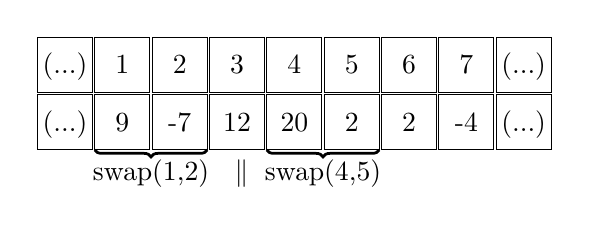
\begin{tikzpicture}[decoration={brace}]
			\matrix (heap) [table, text width=7mm, name=h]
				{ (...) &  1 &  2 &  3 &  4 &  5 &  6 &  7 & (...) \\
				  (...) &  9 & -7 & 12 & 20 &  2 &  2 & -4 & (...) \\};
			\draw [decorate, line width=1pt] (h-2-3.south east) -- (h-2-2.south west)
				node [midway, yshift=-0.3cm, name=t1] {swap(1,2)};
			\node (t2) [right of=t1, xshift=0.15cm] {$\parallel$};
			\draw [decorate, line width=1pt] (h-2-6.south east) -- (h-2-5.south west)
				node [midway, yshift=-0.3cm] {swap(4,5)};
			\end{tikzpicture}
		\end{exampleblock}
		\begin{block}{\emph{Concurrency Rule}}
			\begin{prooftree}
				\AxiomC{$\{Q_1\}C_1\{R_1\}\parallel\cdots\parallel\{Q_n\}C_n\{R_n\}$}
				\UnaryInfC{$\{Q_1\ast\cdots\ast Q_n\}C_1\parallel\cdots\parallel C_n\{R_1\ast\cdots\ast R_n\}$}
			\end{prooftree}
			$$\forall i\neq j.(\textit{free}(Q_i)\cup\textit{free}(R_i))\cap\textit{modifies}(C_j) = \emptyset$$
		\end{block}
	\end{frame}

	\begin{frame}[fragile]
	\frametitle{Mutually-exclusive access}
	\begin{itemize}
		\item provide mutually-exclusive region
		\item specify \emph{resources} for which access is needed
	\end{itemize}
	\begin{block}{\emph{Conditional Critical Region(CCR)}}
	\begin{minipage}{0.35\textwidth}
	\begin{lstlisting}[mathescape]
	with $b$
	when $G$ do
	  $C$
	od;
	\end{lstlisting}
	\end{minipage}\noindent
	\begin{minipage}{0.65\textwidth}
		\begin{enumerate}
			\item aquire $b$
			\item evaluate $G$
			\item if \textit{true} $\rightarrow$ execute $C$
			\item \textit{otherwise} $\rightarrow$ release $b$ and go to 1.
		\end{enumerate}
	\end{minipage}
	\end{block}
	\end{frame}

	\begin{frame}[fragile]
	\frametitle{\emph{CCR-Rule}}
	\begin{itemize}
		\item $\mapsto$ is visibility
		\item only access resources from $b$ within \emph{CCR}
		\item invariant $I_b$ for every \emph{bundle} $b$
	\end{itemize}
	\begin{block}{\emph{CCR-Rule}}
		\begin{prooftree}
			\AxiomC{$\{(Q\ast I_b)\land G\}C\{R\ast I_b\}$}
			\UnaryInfC{$\{Q\}\textit{with $b$ when $G$ do $C$ od}\{R\}$}
		\end{prooftree}
	\end{block}
	\end{frame}

\section{Permission Accounting}
	\subsection{Theoretical Approach}
	\begin{frame}
	\frametitle{Reconsider \emph{Heap}}
	\begin{itemize}
		\item to this point: \emph{Heap} as addressable cells
		\item further abstraction possible
		\item idea: $\mapsto$ decorated with permissions
		\item sound modification
	\end{itemize}
	\begin{block}{\emph{Heap with Permissions}}
		$$h: L \rightharpoonup (V \times M)$$
		\vspace{-0.7cm}
		\begin{itemize}
			\item \emph{addresses}: $L$
			\item \emph{values}: $V$
			\item \emph{permissions}: $M$
		\end{itemize}
	\end{block}
	\end{frame}

	\begin{frame}
	\frametitle{Concept: Permissions}
	\begin{itemize}
		\item either \underline{one} \emph{source permission}
		\item or \underline{multiple} \emph{read permission}
		\item derive \emph{read permissions} from \emph{source permission}
		\item recombine \underline{all} \emph{read permissions} to \emph{source permission}
	\end{itemize}
	\end{frame}

	\begin{frame}
	\frametitle{Permission Set}
	\begin{itemize}
		\item distinguish \emph{source permission} and \emph{read permission}
		\item exactly one unique element $m_W$ as \emph{source permission}
		\item $\oplus$ as operator to split and recombine permissions
	\end{itemize}
	\begin{block}{Source Permission}
		$\exists^{=1}m_W\in M$ with:
		$$\forall m\in M. m_W\oplus m\text{ is undefined.}$$
		$$\forall m\in M\setminus\{m_W\} \exists m'\in M. m\oplus m' = m_W$$
	\end{block}
	\end{frame}

	\begin{frame}
	\frametitle{Permissions in $V\times M$}
	\begin{itemize}
		\item permissions for read access can be recombined
		\item only one value for each cell
	\end{itemize}
	\begin{block}{Permissions in $V\times M$}
		$$(v, m)\oplus(v', m') =
			\begin{cases}
				(v, m\oplus m') &\text{ if }v = v'\text{ and }m\oplus m'\text{ defined} \\
				\textit{undefined} &\text{ otherwise}\\
			\end{cases}
		$$
	\end{block}
	\end{frame}

	\begin{frame}
	\frametitle{Permissions in \emph{Heaps}}
	\begin{itemize}
		\item cell can be part of multiple \emph{Heaps}
		\item agree on value
		\item recombined accordingly
	\end{itemize}
	\begin{block}{Permissions in \emph{Heaps}}
		$$ (h\ast h')(l) =
		\begin{cases}
			h(l)              &\text{if $h'(l)$ is undefined}\\
			h'(l)             &\text{if $h(l) $ is undefined}\\
			h(l) \oplus h'(l) &\text{otherwise}\\
		\end{cases}
		$$
	\end{block}
	\end{frame}

	\begin{frame}[fragile]
	\frametitle{Intuition on \emph{Permissions}}
	\begin{lstlisting}[mathescape]
		(...)
		// source permission on $x$
		[x] := [x] + 1;
		// split up permission on $x$
		//  to two read permissions
		y := [x]; $\parallel$ z := [x];
		// recombine permissions
		//  to one source permission again
		(...)
	\end{lstlisting}
	\end{frame}

	\begin{frame}
	\frametitle{New Axioms}
	\begin{minipage}{0.5\textwidth}
		\begin{itemize}
			\item \emph{source permission}:
			\begin{itemize}
				\item disposing
				\item writing
				\item newly allocated
			\end{itemize}
		\end{itemize}
	\end{minipage}\noindent
	\begin{minipage}{0.5\textwidth}
		\begin{itemize}
			\item \emph{read permission}:
			\begin{itemize}
				\item reading
			\end{itemize}
		\end{itemize}
	\end{minipage}
	\begin{center}
	\begin{tabular}{p{4cm}p{3cm}p{2.4cm}}
		$\{E\xmapsto{m_W}-\}$ & $[E'] := E$ & $\{E'\xmapsto{m_W}E\}$ \\
		\hline
		$\{E\xmapsto{m} n \land \llbracket x\rrbracket s =v\}$ & $x:=[E]$ & $\{E[v/x]\xmapsto{m}n$\\
		&&\hspace{0.5cm}$\land\llbracket x\rrbracket s = n\}$\\
		\hline
		$\{\textit{emp}\}$ & $x:=\textit{new}()$ & $\{x \xmapsto{m_W} -\}$\\
		\hline
		$\{E\xmapsto{m_W}-\}$ & $\textit{dispose}(E)$ & $\{\textit{emp}\}$\\
	\end{tabular}
	\end{center}

	\end{frame}


	\subsection{Fractional Permissions}
	\begin{frame}
	\frametitle{Idea: \emph{Fractional Permissions}}
	\begin{itemize}
		\item definition of a set $M$ and operator $\oplus$ yields model
		\item example \emph{Fractional Permissions}:
		\begin{itemize}
			\item \emph{source permission} is one whole permission (i.e. 1)
			\item permission locally divisible into two \emph{read permissions} (i. e. fractions)
			\item recombining by adding up fractions
		\end{itemize}
	\end{itemize}
	\vspace{-0.1cm}
	\begin{block}{\emph{Fractional Permissions}}
		\vspace{-0.4cm}
		\begin{minipage}{0.35\textwidth}
			$$M = (0,1]\cap\mathbb{Q}$$
			$$m_W = 1$$
		\end{minipage}\noindent
		\begin{minipage}{0.65\textwidth}
			$$z\oplus_\text{FP} z' =
			\begin{cases}
				\textit{undefined} &\text{if $z + z' > 1$}\\
				z + z'             &\text{otherwise}\\
			\end{cases}
			$$
		\end{minipage}
	\end{block}
	\end{frame}

	\begin{frame}[fragile]
	\frametitle{Example: Application of \emph{Fractional Permissions}}
	\begin{exampleblock}{Concurrent Map on Tree\footnotemark}
	\begin{center}
	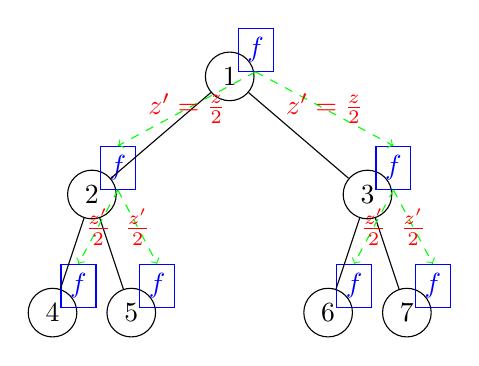
\begin{tikzpicture}[level distance=1.5cm,
	level 1/.style={sibling distance=3.5cm},
	level 2/.style={sibling distance=1cm},
	label distance=-2mm]
	\tikzstyle{every node}=[circle,draw]

		\node [label={[name=m1, rectangle, draw, blue, visible on=<2-3>]30:$f$}] (Root) {1}
		child {
			node [label={[name=m2, rectangle, draw, blue, visible on=<3-5>]30:$f$}] {2} 
			child { node [label={[name=m4, rectangle, draw, blue, visible on=<5-6>]30:$f$}] {4} }
			child { node [label={[name=m5, rectangle, draw, blue, visible on=<5-6>]30:$f$}] {5} }
		}
		child {
			node [label={[name=m3, rectangle, draw, blue, visible on=<3-5>]30:$f$}] {3}
			child { node [label={[name=m6, rectangle, draw, blue, visible on=<5-6>]30:$f$}] {6} }
			child { node [label={[name=m7, rectangle, draw, blue, visible on=<5-6>]30:$f$}] {7} }
	};
	\draw<3-3> [dashed, ->, green] (m1.south) -- (m2.north) node [red, midway,draw=none, rectangle] {$z' = \frac{z}{2}$};
	\draw<3-3> [dashed, ->, green] (m1.south) -- (m3.north) node [red, midway,draw=none, rectangle] {$z' = \frac{z}{2}$};
	\draw<5-5> [dashed, ->, green] (m2.south) -- (m4.north) node [red, midway,draw=none, rectangle] {$\frac{z'}{2}$};
	\draw<5-5> [dashed, ->, green] (m2.south) -- (m5.north) node [red, midway,draw=none, rectangle] {$\frac{z'}{2}$};
	\draw<5-5> [dashed, ->, green] (m3.south) -- (m6.north) node [red, midway,draw=none, rectangle] {$\frac{z'}{2}$};
	\draw<5-5> [dashed, ->, green] (m3.south) -- (m7.north) node [red, midway,draw=none, rectangle] {$\frac{z'}{2}$};

	\end{tikzpicture}
	\end{center}
	\end{exampleblock}
	\footnotetext[1]{\tiny Analogue to \emph{Lambda-term substitution} in \emph{Permission Accounting in Separation Logic}.}
	\end{frame}

	\section{Conclusion}
	\begin{frame}
	\frametitle{Conclusion}
	\begin{itemize}
		\item \emph{Separation Logic} extends \emph{Hoare Calculus}
		\item reasoning about
		\begin{itemize}
			\item mutable data structures in the \emph{Heap}
			\item concurrent programs
		\end{itemize}
		\item \emph{Permission Accounting} to manage access to shared memory
		\begin{itemize}
			\item multiple models possible
		\end{itemize}
		\item related research:
		\begin{itemize}
			\item permissions for \emph{Stores}
			\item use in verification tool, e.g. \emph{smallfoot}
		\end{itemize}
	\end{itemize}
	\end{frame}

	\begin{frame}[allowframebreaks]
	\frametitle<presentation>{Sources}
		\emph{Hoare Calculus:}
		\begin{thebibliography}{}
		\bibitem{hoarecalc}
			C.~A.~R.~Hoare
			\newblock An Axiomatic Basis for Computer Programming
			\newblock \emph{Commun. ACM, 12(10):576-580, 1969.}

		\end{thebibliography}

		\vspace{0.3cm}
		\emph{Separation Logic:}
		\begin{thebibliography}{}
		\bibitem{Primer}
			P.~O'Hearn
			\newblock A Primer on Separation Logic (and Automatic Program Verification and Analysis)
			\newblock \emph{NATO Science for Peace and Security Series, Sub-series D: Information and Communication Security, 33:286-318, 2012.}
		
		\bibitem{ConcurrencyInSepLogic}
			P.~O'Hearn
			\newblock Resources, Concurrency, and Local Reasoning
			\newblock \emph{Theor. Comp. Sci. 375(1-3):271-307, 2007.}

		\end{thebibliography}

		\vspace{0.3cm}
		\emph{Permission Accounting:}
		\begin{thebibliography}{}

		\bibitem{PermAcc}
			R.~Bornat, C.~Calgano, P.~O'Hearn and M.~Parkinson
			\newblock Permission Accounting in Separation Logic
			\newblock \emph{SIGPLAN Not., 40(1):259-270, 2005.}

		\bibitem{freshlook}
			R.~Dockins, H.~Aquinas and A.~Appel
			\newblock A Fresh Look at Separation Algebras and Share Accounting
			\newblock \emph{Proceedings of the 7th Asian Symposium on Programming Languages and Systems, APLAS '09, pages 161-177, Springer-Verlag, 2009.}

		\bibitem{sembasis}
			H.~Yang and P.~O'Hearn
			\newblock A Semantic Basis for Local Reasoning
			\newblock \emph{Proceedings of the 5th International Conference on Foundations of Software Science and Computation Structures, FoSSaCS '02, pages 402-416, Springer Verlag, 2002.}

		\bibitem{seplogproof}
			C.~Calcagno, P.~O'Hearn and H.~Yang
			\newblock Local Action and Abstract Separation Logic
			\newblock \emph{Proceedings of the 22nd Annual IEEE Symposium on Logic in Computer Science, LICS '07, pages 366-378, IEEE Computer Society, 2007.}

		\end{thebibliography}

		\vspace{0.3cm}
		\emph{Further Research:}
		\begin{thebibliography}{}

		\bibitem{storeperm}
			S.~Brookes
			\newblock Variables as Resource for Shared-Memory Programs: Semantics and Soundness
			\newblock \emph{Electronic Notes in Theoretical Computer Science, 158(0):123-150, 2006.}
		\end{thebibliography}
	\end{frame}

	\begin{frame}
		\frametitle{The End}
		\begin{center}
			\huge{Thank you for your attention.}
		\end{center}
	\end{frame}

% backup:
	\begin{frame}
	\frametitle{Idea: \emph{Counting Permissions}}
	\begin{itemize}
		\item one distinguishable \emph{source permission}
		\begin{itemize}
		\item positive counter
		\end{itemize}
		\item gives away reading tokens
		\begin{itemize}
			\item negativ permission
		\end{itemize}
	\end{itemize}
	\end{frame}

	\begin{frame}[noframenumbering]
	\frametitle{Definition: \emph{Counting Permissions}}
		\begin{block}{Definition}
			\begin{minipage}{0.25\textwidth}
				$$M = \mathbb{Z}$$
				$$m_W = 0$$
			\end{minipage}\noindent
			\begin{minipage}{0.75\textwidth}
				$$z\oplus_\text{CP} z' =
					\begin{cases}
						\text{undefined} & \text{if $z \geq 0$ and $z' \geq 0$}\\
						\text{undefined} & \text{if ($z\geq 0$ or  $z' \geq 0$)}\\
						                 & \text{ and $z + z' < 0$}\\
						z + z'           & \text{otherwise}
					\end{cases}
				$$
			\end{minipage}
		\end{block}
		\begin{exampleblock}{Readers-Writers Problem}
			\begin{itemize}
				\item one writer
				\item multiple reader
				\item count variable for reader
			\end{itemize}
		\end{exampleblock}
	\end{frame}

	\begin{frame}[noframenumbering]
	\frametitle{Boolean Permission Model}
		\begin{itemize}
			\item $M = \{\textit{true}, \textit{false}\}$
			\item drop all cells which are not seen
			\item equivalent to \emph{Heap} without \emph{Permissions}
		\end{itemize}
	\end{frame}

	\begin{frame}[noframenumbering]
	\frametitle{Properties of \emph{Permission Models}}
		\begin{itemize}
			\item \emph{Cross-Split}: if 2 ways exist to split, 4 ways exist
			\item \emph{Splittability}: a \emph{permission} can be infinitly split
		\end{itemize}
	\end{frame}

	\begin{frame}[fragile, noframenumbering]
	\frametitle{Implementation of Concurrent Tree Map}
	\begin{lstlisting}[mathescape]
	map (f, t) {
	  if isLeaf (t) {
	    skip;
	  } else {
	    apply ([f], [t.value]);
	    map (f, t.left); $\parallel$ map (f, t.right);
	  }
	}
	\end{lstlisting}
	\end{frame}

	\begin{frame}[noframenumbering]
	\frametitle{Resources Bundle}
	\begin{quote}
		Hoare called resource bundles simply resources, but I
		want that word to apply to the items - heap locations
		and variables at least, perhaps time and stack space
		and whatever else we can manage - and the permissions
		that are owned by, shared between or transferred between
		the threads of a concurrent program.
	\end{quote}
	- R.~Bornat, C.~Calcagno, P.~O'Hearn, and M.~Parkinson. Permission Accounting
	in Separation Logic. \textit{SIGPLAN Not.}, 40(1):259-270, 2005.
	\end{frame}

\end{document}
